This section will present the findings of our experiments.
The two measures used to compare our methods are the change in loss and the change in accuracy.
The difference between the benchmarked model and our mutated models is compared to evaluate the trained model.
We compare the loss and accuracy of the benchmark model at a further epoch to the run epoch of our algorithm.
For the non-expert runs, we use the standard model benchmark.
\subsection{Impact of Training on Mutated Models}\label{subsec:impact-of-training-on-mutated-models}
Our models \ref{fig:loss-accuracy-training} show slightly better loss and accuracy than the benchmark during training.
However, we observed a drop in both metrics after the 12th epoch for loss and after the 11th epoch for accuracy.

The figure \ref{fig:decay_training} displays the number of trained models.
It appears that the break condition was not met in the previous epoch.
By the 6th epoch, the number of running models had already been halved.
At the 10th epoch, only one-fifth of the original runs remain.
Therefore, for subsequent analysis, we will only consider data points with an epoch of 10 or less.
\begin{figure}
    \centering
    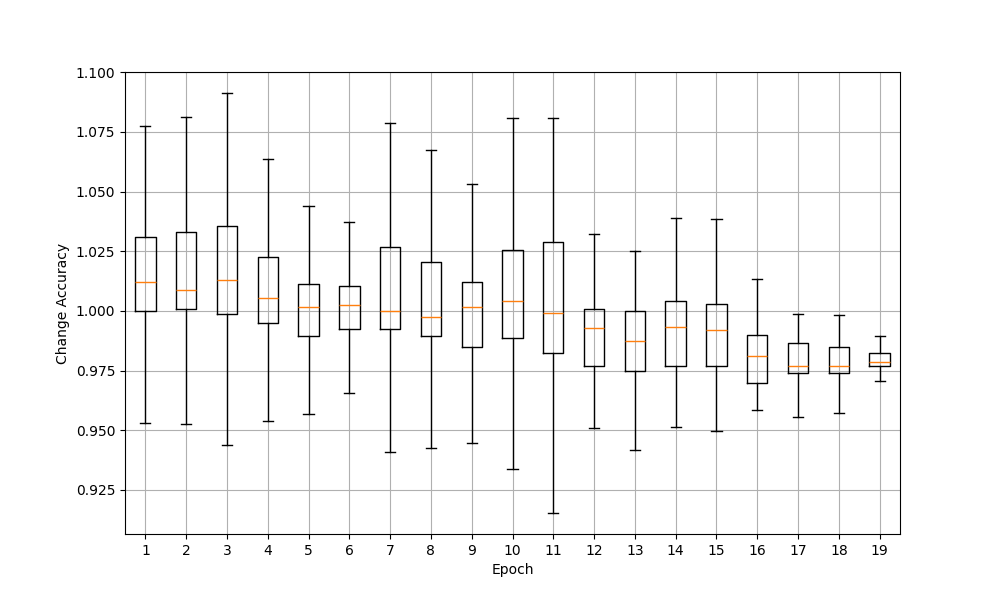
\includegraphics[width=\textwidth]{plots/Trained_Change_Acc.png}
    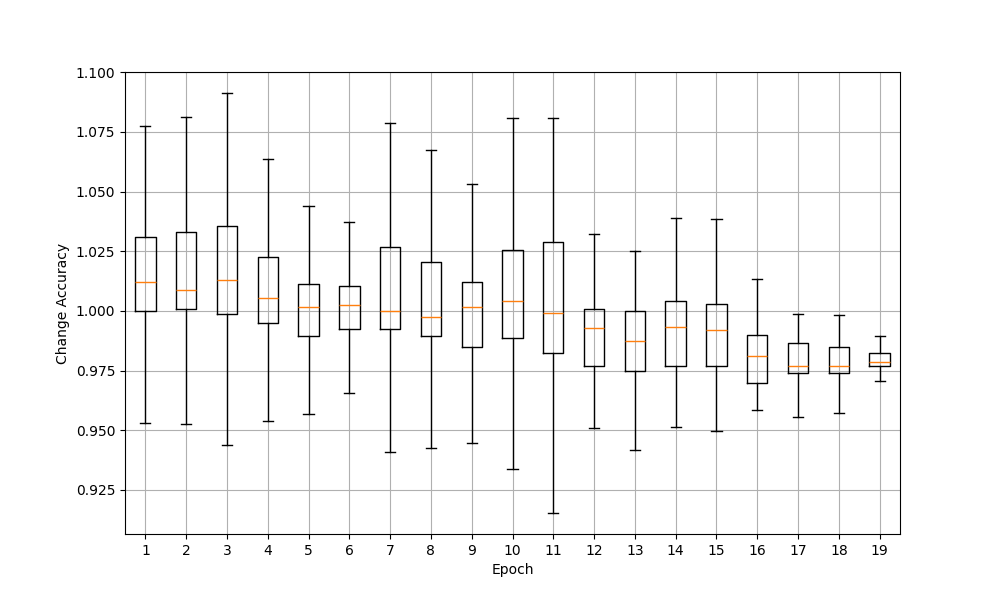
\includegraphics[width=\textwidth]{plots/Trained_Change_Loss.png}
    \caption{Loss and accuracy of the models, with training}
    \label{fig:loss-accuracy-training}
\end{figure}
\begin{figure}
    \centering
    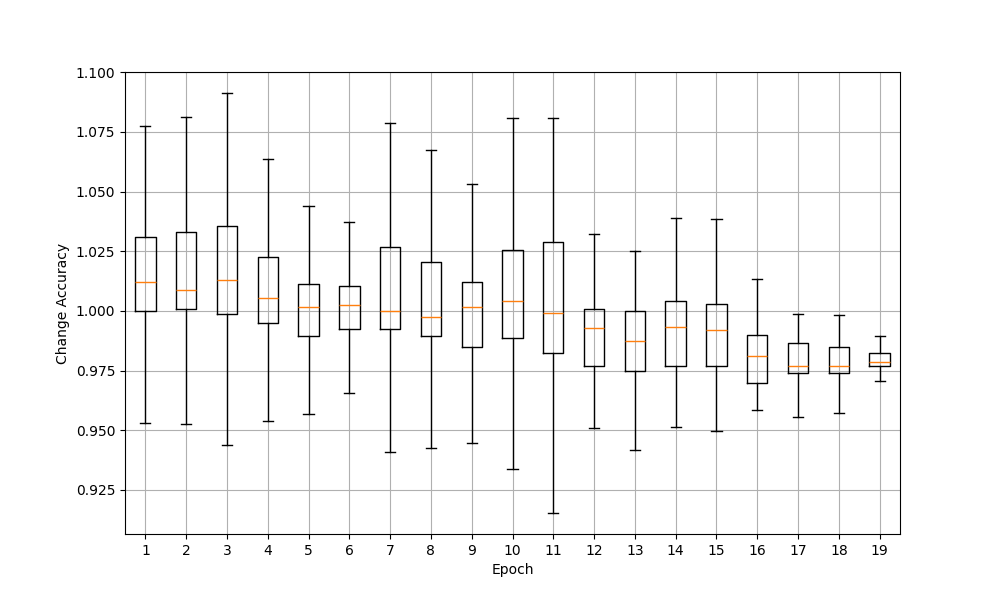
\includegraphics[width=\textwidth]{plots/Trained_Points_perEpoch.png}
    \caption{Decay of data points, per epoch, with training}
    \label{fig:decay_training}
\end{figure}
\subsection{Effects of Mutation Without Training}\label{subsec:effects-of-mutation-without-training}
For the models \ref{fig:loss-accuracy-Notraining}, there is a significant improvement in accuracy and loss during the first three epochs.
However, after that, the values remain close to the baseline of 1.

The figure \ref{fig:decay_Notraining} shows the number of trained models.
The break condition was not met in the previous epoch.
Additionally, we observe that after 5 epochs, only a quarter of the runs remain, and after 10 epochs, only an eighth remains.
Based on these results, we decided to focus on data points with an epoch of 5 or less.
\begin{figure}
    \centering
    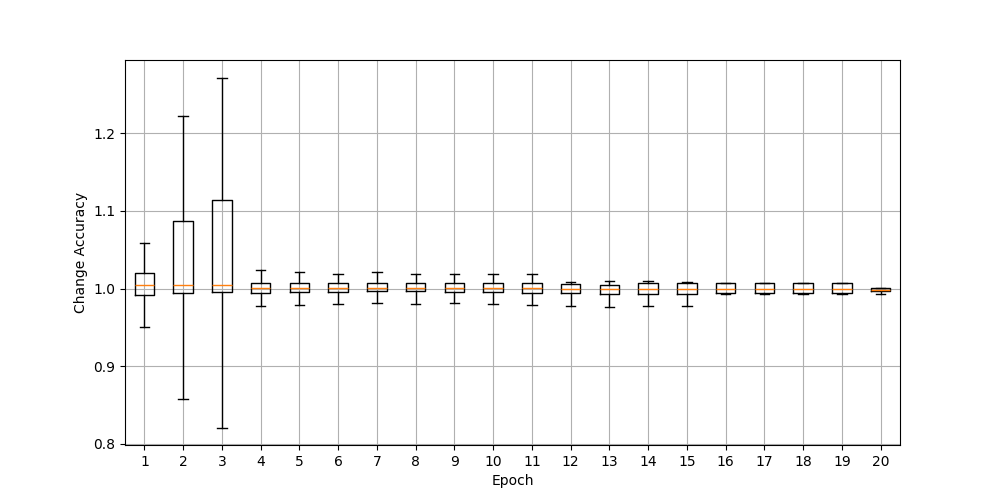
\includegraphics[width=\textwidth]{plots/NotTrained_Change_Acc.png}
    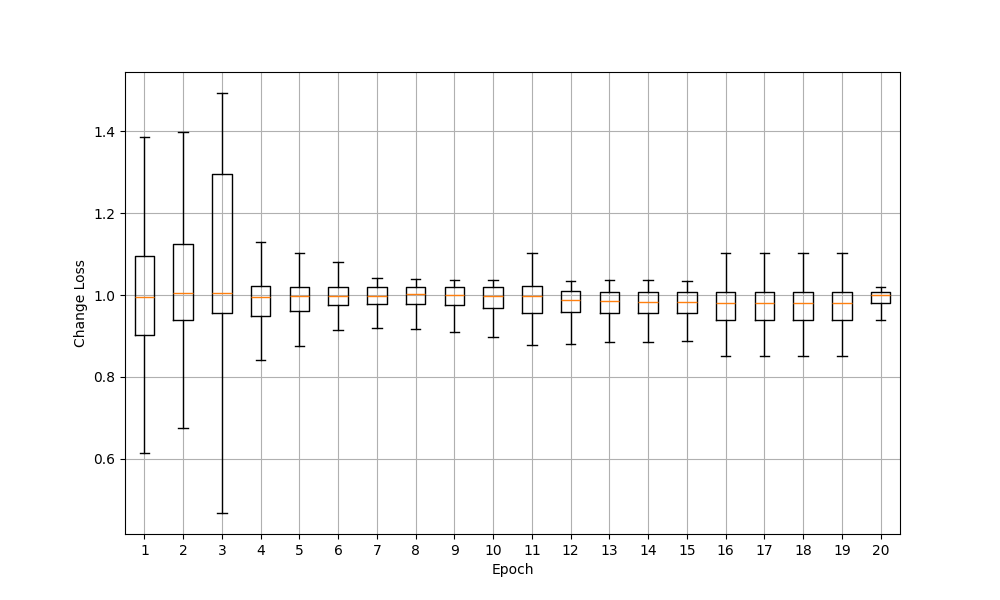
\includegraphics[width=\textwidth]{plots/NotTrained_Change_Loss.png}
    \caption{Loss and accuracy of the models, without training}
    \label{fig:loss-accuracy-Notraining}
\end{figure}
\begin{figure}
    \centering
    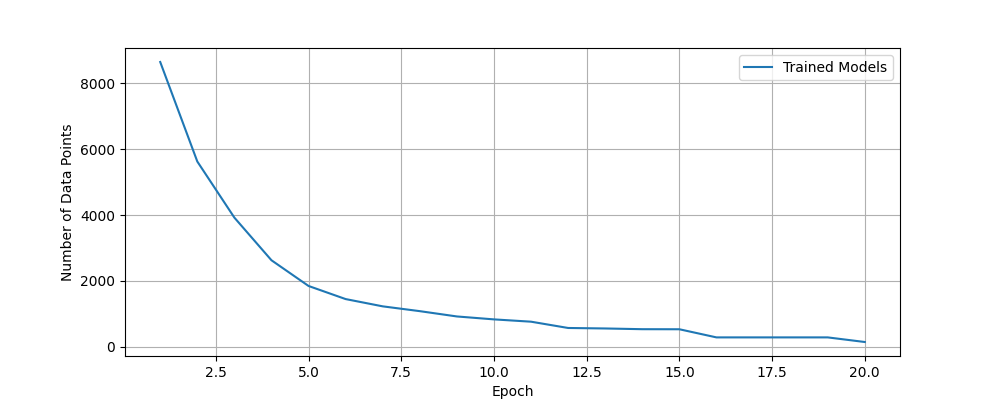
\includegraphics[width=\textwidth]{plots/NotTrained_Points_perEpoch.png}
    \caption{Decay of data points, per epoch, without training}
    \label{fig:decay_Notraining}
\end{figure}
\subsection{Effects of the extend of pre Training}\label{subsec:effects-of-the-extend-of-pre-training}
The initial epoch 1 shows \ref{fig:initial-epochs-notraining} a significant improvement in both loss and accuracy for the execution without training.
However, this improvement is not observed in models with 6 initial epochs.

In contrast, when executing the model \ref{fig:initial-epochs-training} with training, the most promising model remains the one with 1 initial epoch.
However, models with an initial 6 epochs still produce better results.
Due to the poor results of the non-trained 6 initial epoch models, we decided to focus solely on models with 1 initial epoch for further investigation.
\begin{figure}
    \begin{subfigure}{0.5\textwidth}
        \centering
        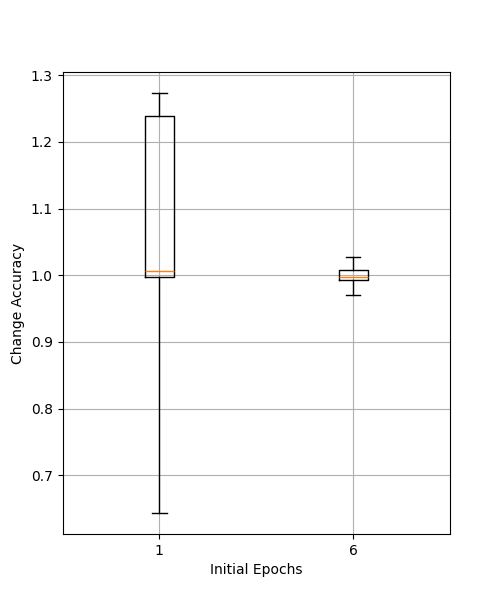
\includegraphics[width=0.95\textwidth]{plots/InitEpoch_NotTrained_accuracy.png}
    \end{subfigure}
    \begin{subfigure}{0.5\textwidth}
        \centering
        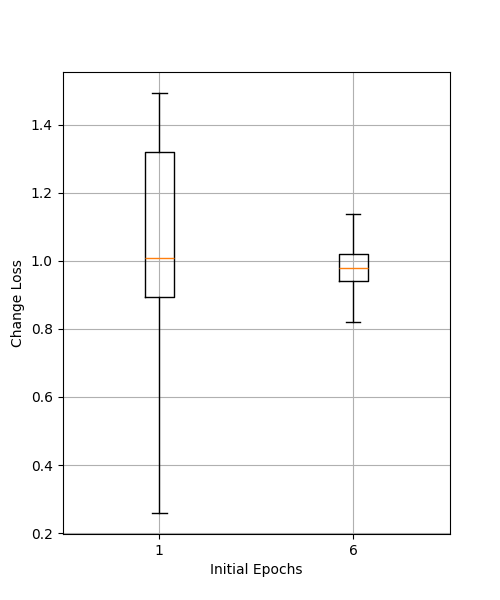
\includegraphics[width=0.95\textwidth]{plots/InitEpoch_NotTrained_loss.png}
    \end{subfigure}
    \caption{Loss and accuracy, without training, with different initial epochs}
    \label{fig:initial-epochs-notraining}
\end{figure}
\begin{figure}
    \begin{subfigure}{0.5\textwidth}
        \centering
        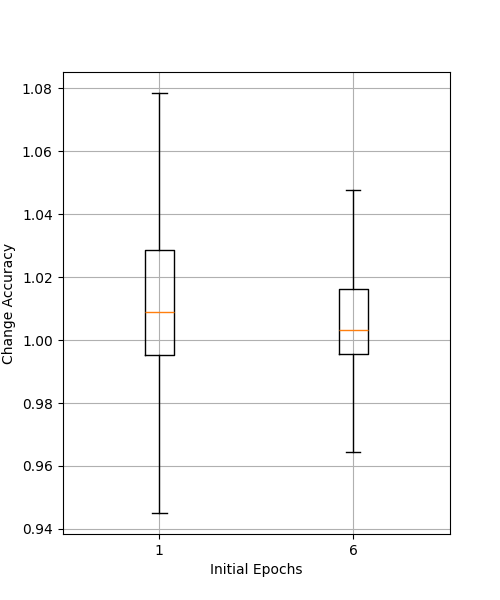
\includegraphics[width=0.95\textwidth]{plots/InitEpoch_Trained_accuracy.png}
    \end{subfigure}
    \begin{subfigure}{0.5\textwidth}
        \centering
        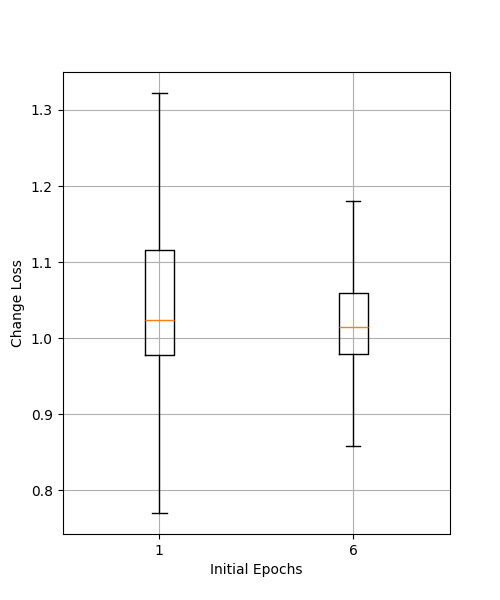
\includegraphics[width=0.95\textwidth]{plots/InitEpoch_Trained_loss.png}
    \end{subfigure}
    \caption{Loss and accuracy, with training, with different initial epochs}
    \label{fig:initial-epochs-training}
\end{figure}
\subsection{Training Dataset Size and Model Performance}\label{subsec:training-dataset-size-and-model-performance}
When examining the datasets without training \ref{fig:dataset-size-notraining}, we observe similar accuracies for both the full and half datasets.
However, the loss is slightly worse for the half dataset compared to the full dataset.
For the trained runs \ref{fig:dataset-size-training}, there is a greater distance between the full and half datasets.
For both with and without training, we see not very promising results for the quarter dataset.
\begin{figure}
    \begin{subfigure}{0.5\textwidth}
        \centering
        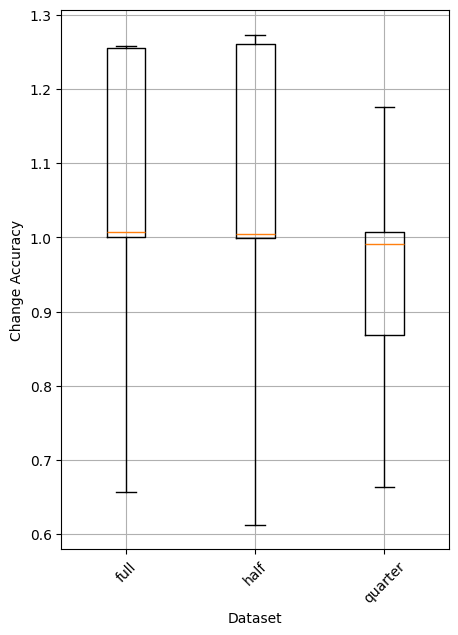
\includegraphics[width=0.95\textwidth]{plots/Dataset_NotTrained_accuracy.png}
    \end{subfigure}
    \begin{subfigure}{0.5\textwidth}
        \centering
        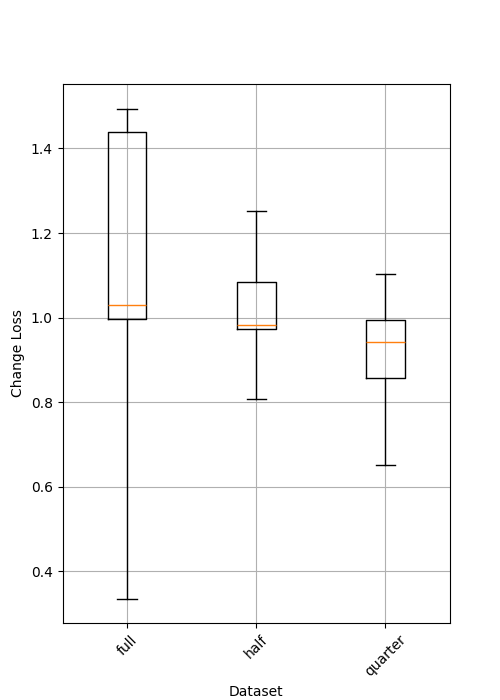
\includegraphics[width=0.95\textwidth]{plots/Dataset_NotTrained_loss.png}
    \end{subfigure}
    \caption{Loss and accuracy, without training, with different dataset sizes}
    \label{fig:dataset-size-notraining}
\end{figure}
\begin{figure}
    \begin{subfigure}{0.5\textwidth}
        \centering
        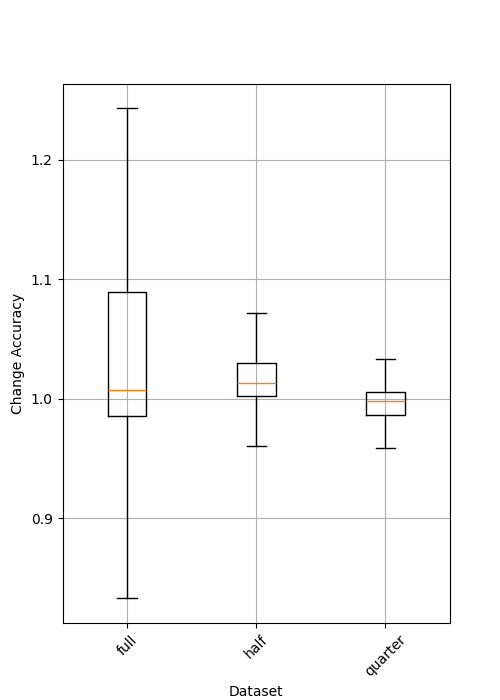
\includegraphics[width=0.95\textwidth]{plots/Dataset_Trained_accuracy.png}
    \end{subfigure}
    \begin{subfigure}{0.5\textwidth}
        \centering
        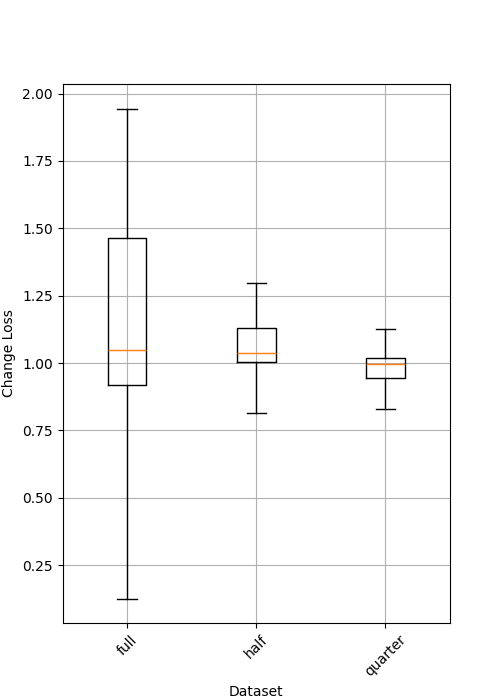
\includegraphics[width=0.95\textwidth]{plots/Dataset_Trained_loss.png}
    \end{subfigure}
    \caption{Loss and accuracy, with training, with different dataset sizes}
    \label{fig:dataset-size-training}
\end{figure}
\subsection{Influence of Suspiciousness Measures}\label{subsec:influence-of-suspiciousness-measures}
For both trained \ref{fig:suspiciousness-measures-training} and untrained runs \ref{fig:suspiciousness-measures-notraining}, Tarantula appears to be the most promising measure of suspiciousness.
In contrast to expectations, Random only reliably exceeded in the runs without training.
There is no discernible difference between each random choosing, ochiai, and dstar in the trained runs.
For runs without training, ochiai appears to be superior to dstar and random selection.
\begin{figure}
    \begin{subfigure}{0.5\textwidth}
        \centering
        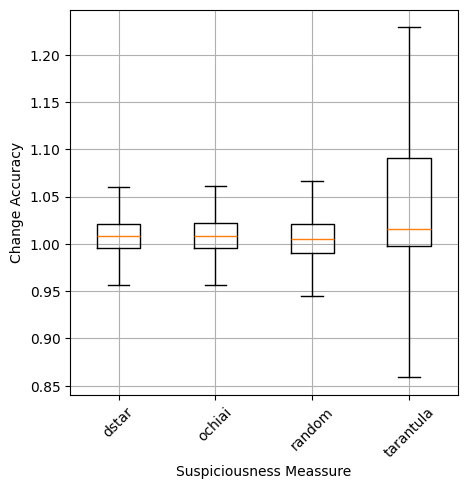
\includegraphics[width=0.95\textwidth]{plots/Meassure_Trained_accuracy.png}
    \end{subfigure}
    \begin{subfigure}{0.5\textwidth}
        \centering
        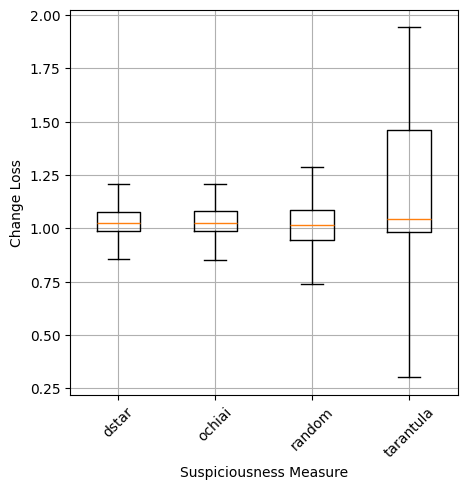
\includegraphics[width=0.95\textwidth]{plots/Meassure_Trained_loss.png}
    \end{subfigure}
    \caption{Loss and accuracy, with training, with different suspiciousness measures}
    \label{fig:suspiciousness-measures-training}
\end{figure}
\begin{figure}
    \begin{subfigure}{0.5\textwidth}
        \centering
        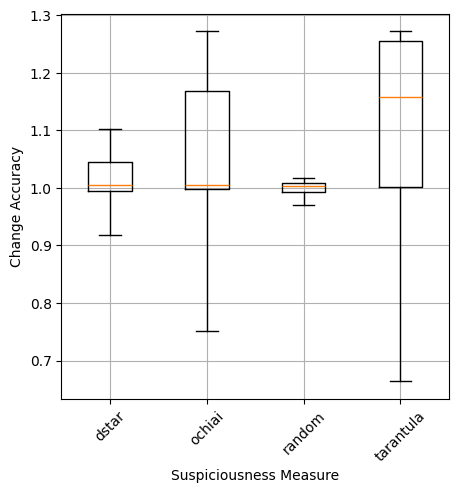
\includegraphics[width=0.95\textwidth]{plots/Meassure_NotTrained_accuracy.png}
    \end{subfigure}
    \begin{subfigure}{0.5\textwidth}
        \centering
        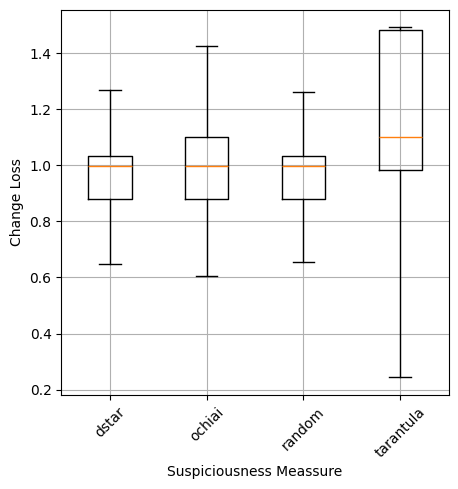
\includegraphics[width=0.95\textwidth]{plots/Meassure_NotTrained_loss.png}
    \end{subfigure}
    \caption{Loss and accuracy, without training, with different suspiciousness measures}
    \label{fig:suspiciousness-measures-notraining}
\end{figure}
\subsection{CNN vs. DNN Architectural Efficiency}\label{subsec:cnn-vs.-dnn-architectural-efficiency}
For both the trained \ref{fig:architecture-notraining} and untrained \ref{fig:architecture-training} runs, CNN1 appears to be the most promising architecture, while CNN2 shows promise for untrained runs in terms of accuracy but performs poorly in terms of loss.
For both trained and non-trained runs, the deep neural networks are not performing better than the baseline.
CNN2 is underperforming in the trained runs.
\begin{figure}
    \begin{subfigure}{0.5\textwidth}
        \centering
        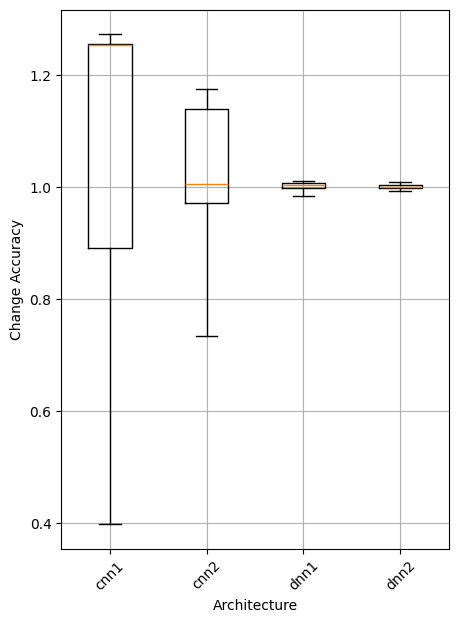
\includegraphics[width=0.95\textwidth]{plots/Architecture_NotTrained_accuracy.png}
    \end{subfigure}
    \begin{subfigure}{0.5\textwidth}
        \centering
        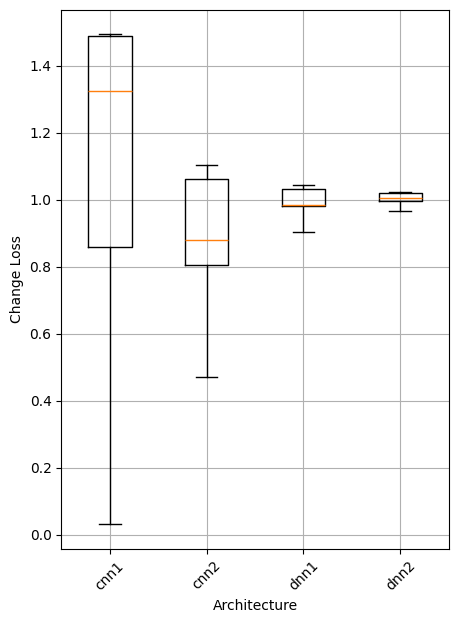
\includegraphics[width=0.95\textwidth]{plots/Architecture_NotTrained_loss.png}
    \end{subfigure}
    \caption{Loss and accuracy, without training, with different architectures}
    \label{fig:architecture-notraining}
\end{figure}
\begin{figure}
    \begin{subfigure}{0.5\textwidth}
        \centering
        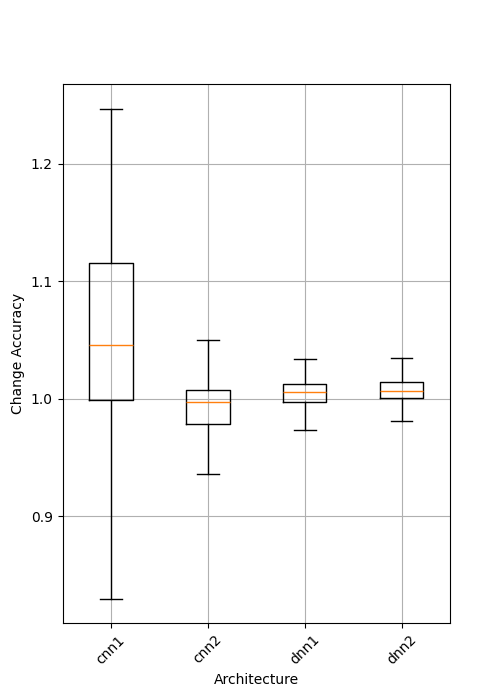
\includegraphics[width=0.95\textwidth]{plots/Architecture_Trained_accuracy.png}
    \end{subfigure}
    \begin{subfigure}{0.5\textwidth}
        \centering
        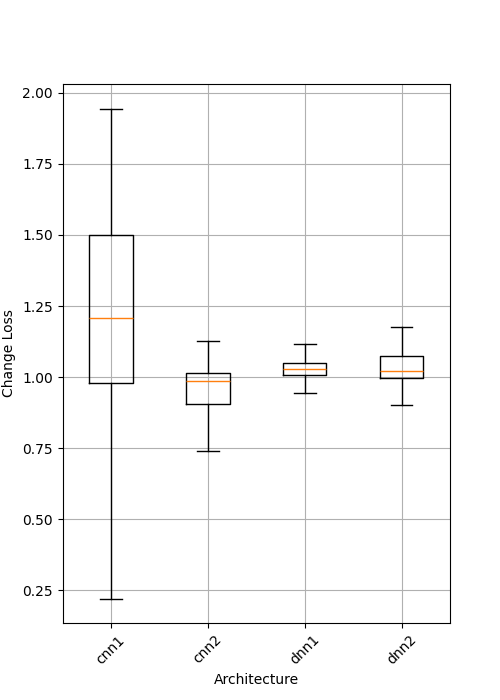
\includegraphics[width=0.95\textwidth]{plots/Architecture_Trained_loss.png}
    \end{subfigure}
    \caption{Loss and accuracy, with training, with different architectures}
    \label{fig:architecture-training}
\end{figure}
\subsection{Offset Variations in Loss and Accuracy}\label{subsec:offset-variations-in-loss-and-accuracy}
Although the median change with and without the offset is similar \ref{fig:offset-training}\ref{fig:offset-notraining}, it is important to note that the upper quartile of the categories uses the offset, as indicated by the data.
This suggests that an offset ultimately produces a better result.
\begin{figure}
    \begin{subfigure}{0.5\textwidth}
        \centering
        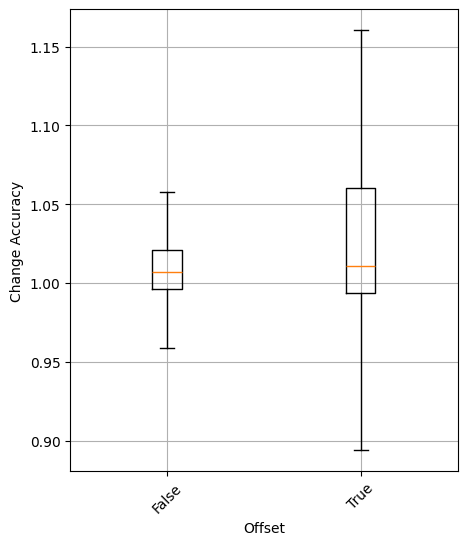
\includegraphics[width=0.95\textwidth]{plots/Offset_Trained_accuracy.png}
    \end{subfigure}
    \begin{subfigure}{0.5\textwidth}
        \centering
        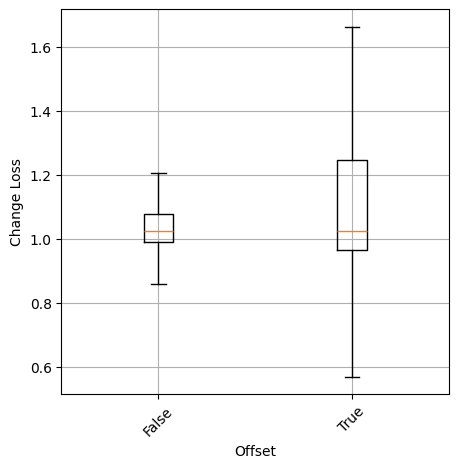
\includegraphics[width=0.95\textwidth]{plots/Offset_Trained_loss.png}
    \end{subfigure}
    \caption{Loss and accuracy, with training, with offsets or not}
    \label{fig:offset-training}
\end{figure}
\begin{figure}
    \begin{subfigure}{0.5\textwidth}
        \centering
        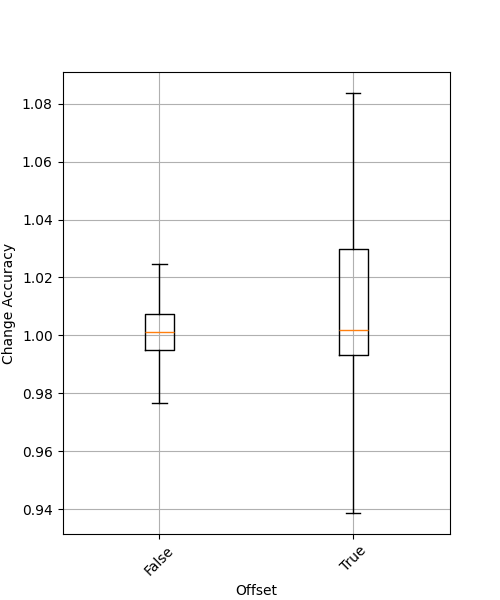
\includegraphics[width=0.95\textwidth]{plots/Offset_NotTrained_accuracy.png}
    \end{subfigure}
    \begin{subfigure}{0.5\textwidth}
        \centering
        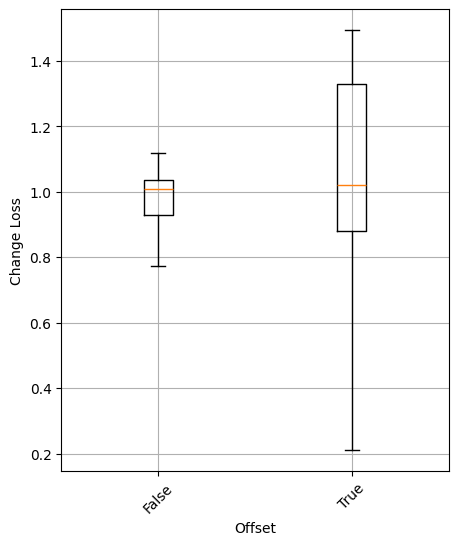
\includegraphics[width=0.95\textwidth]{plots/Offset_NotTrained_loss.png}
    \end{subfigure}
    \caption{Loss and accuracy, without training, with offsets or not}
    \label{fig:offset-notraining}
\end{figure}
\subsection{Break Conditions and Algorithm Performance}\label{subsec:break-conditions-and-algorithm-performance}
There were no significant differences observed \ref{fig:break-conditions-training} among the four options for the different break conditions.
However, some differences were noted in the samples that were not trained \ref{fig:break-conditions-notraining} during the execution of our algorithms.
In terms of accuracy, the most promising comparison appears to be between Accuracy and Loss and Accuracy.
Loss, on the other hand, seems to be neutral.
While Loss or Accuracy still results in a small improvement, it is not as significant as the first two.
For the loss also Accuracy and Loss and Accuracy seem to be the most promising, while Loss and Loss or Accuracy are rather neutral toward worsening.
\begin{figure}
    \begin{subfigure}{0.5\textwidth}
        \centering
        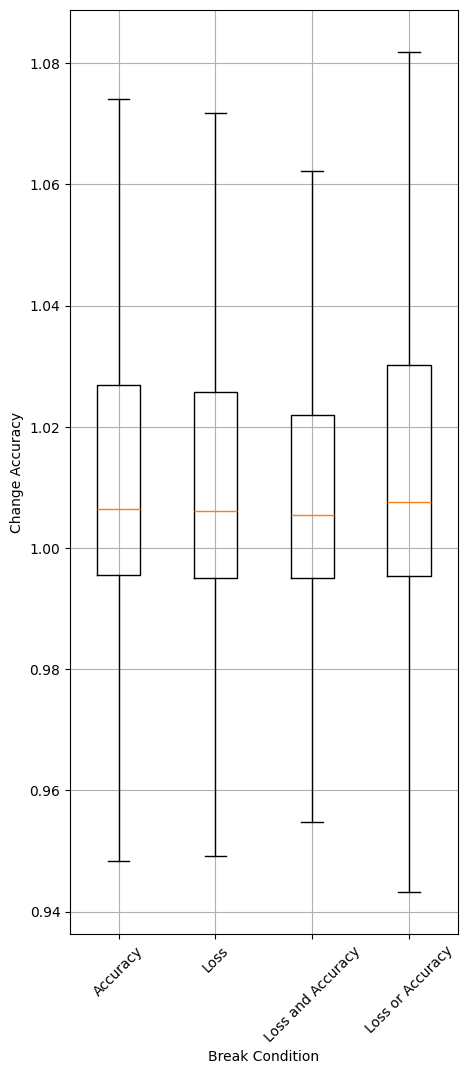
\includegraphics[width=0.95\textwidth]{plots/BreakCondition_Trained_accuracy.png}
    \end{subfigure}
    \begin{subfigure}{0.5\textwidth}
        \centering
        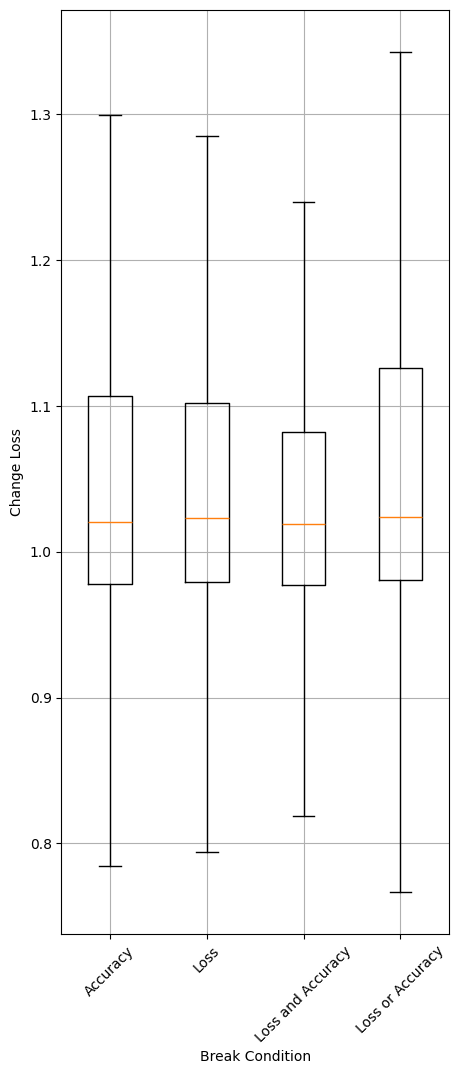
\includegraphics[width=0.95\textwidth]{plots/BreakCondition_Trained_loss.png}
    \end{subfigure}
    \caption{Loss and accuracy, with training, with different break conditions}
    \label{fig:break-conditions-training}
\end{figure}
\begin{figure}
    \begin{subfigure}{0.5\textwidth}
        \centering
        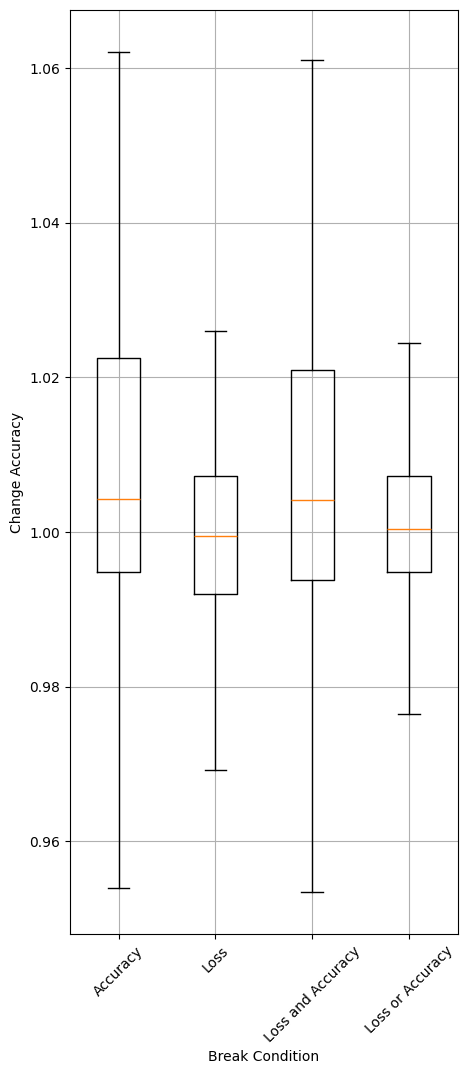
\includegraphics[width=0.95\textwidth]{plots/BreakCondition_NotTrained_accuracy.png}
    \end{subfigure}
    \begin{subfigure}{0.5\textwidth}
        \centering
        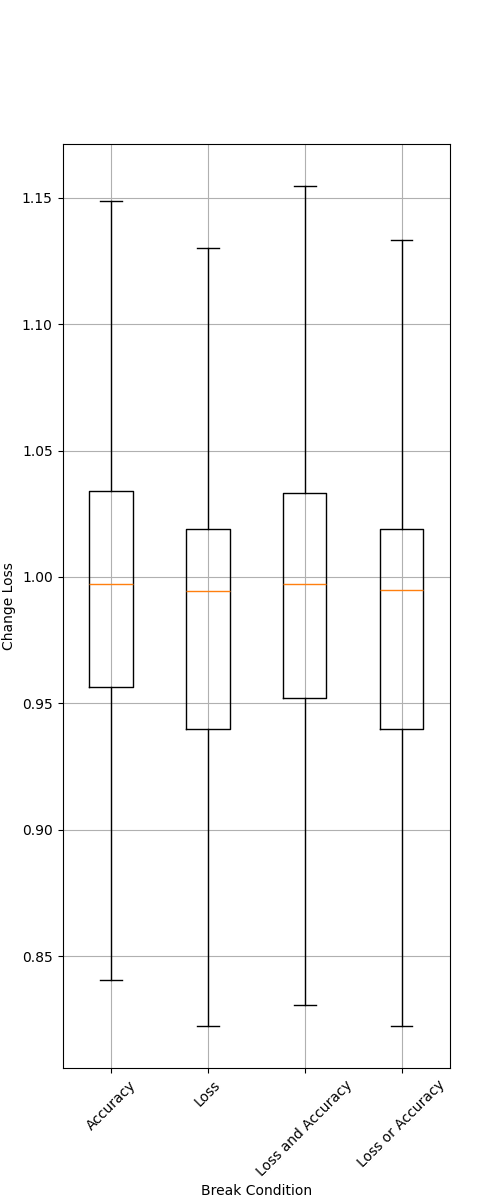
\includegraphics[width=0.95\textwidth]{plots/BreakCondition_NotTrained_loss.png}
    \end{subfigure}
    \caption{Loss and accuracy, without training, with different break conditions}
    \label{fig:break-conditions-notraining}
\end{figure}
\subsection{Contributions of Different Mutation Functions}\label{subsec:contributions-of-different-mutation-functions}
There were no significant differences between the functions examined for the trained runs \ref{fig:mutation-functions-training}, except for \texttt{modify\_weight\_all\_random\_by\_scalar\_gauss} \ref{lst:scalar_weight_mod}, which performed worse in terms of both loss and accuracy.
In contrast, the non-trained \ref{fig:mutation-functions-notraining} runs yielded similar results for the weight modifying functions, but no significant improvements were observed when using bias modifying functions.
\begin{figure}
    \begin{subfigure}{0.5\textwidth}
        \centering
        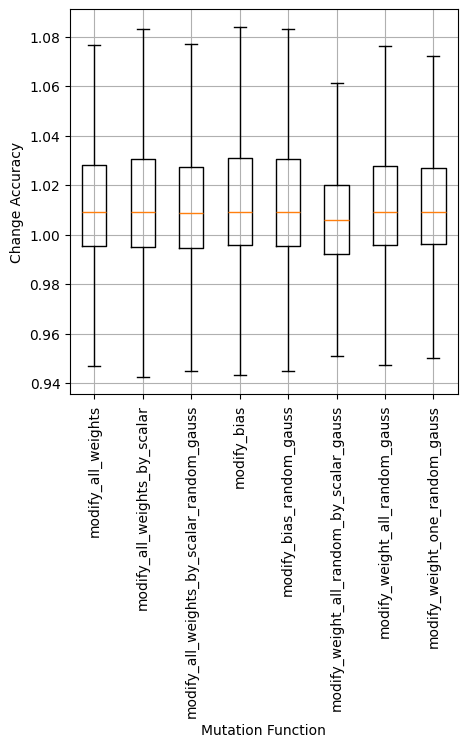
\includegraphics[width=0.95\textwidth]{plots/Mutatation_Trained_accuracy.png}
    \end{subfigure}
    \begin{subfigure}{0.5\textwidth}
        \centering
        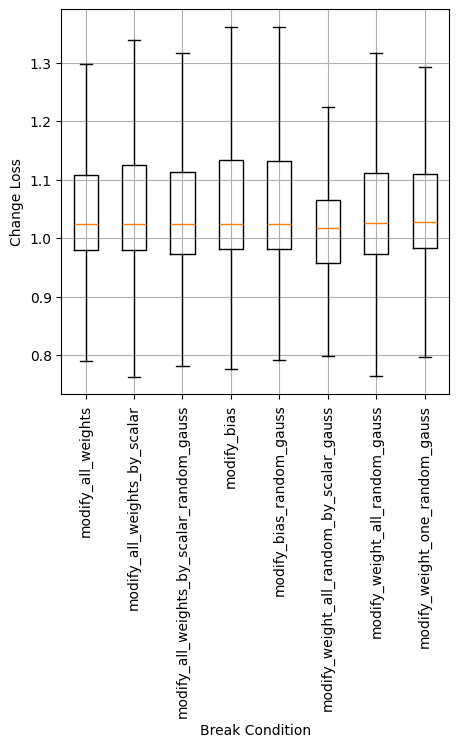
\includegraphics[width=0.95\textwidth]{plots/Mutatation_Trained_loss.png}
    \end{subfigure}
    \caption{Loss and accuracy, with training, with different mutation functions}
    \label{fig:mutation-functions-training}
\end{figure}
\begin{figure}
    \begin{subfigure}{0.5\textwidth}
        \centering
        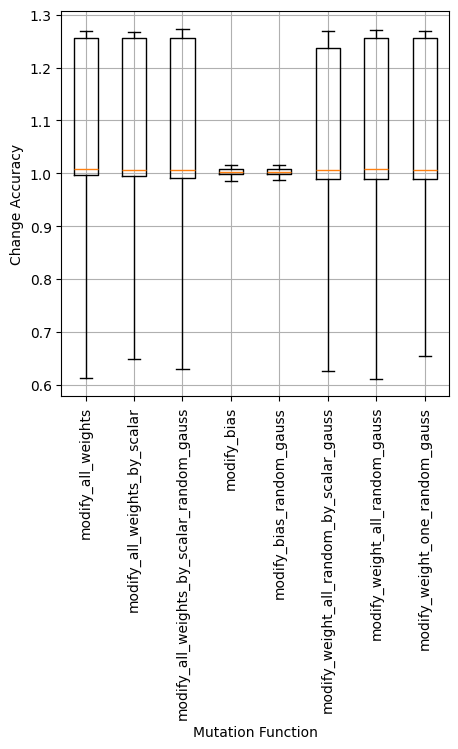
\includegraphics[width=0.95\textwidth]{plots/Mutatation_NotTrained_accuracy.png}
    \end{subfigure}
    \begin{subfigure}{0.5\textwidth}
        \centering
        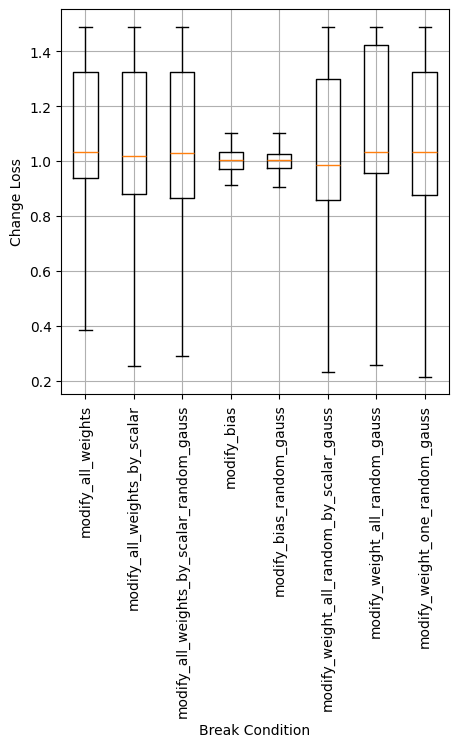
\includegraphics[width=0.95\textwidth]{plots/Mutatation_NotTrained_loss.png}
    \end{subfigure}
    \caption{Loss and accuracy, without training, with different mutation functions}
    \label{fig:mutation-functions-notraining}
\end{figure}